%%%%%%%%%%%%%%%%%%%%%%%%%%%%%%%%%%%%%%%%%%%%%%%%%%%%%%%%
\documentclass[12pt,a4paper]{article}% 文档格式
\usepackage{ctex,hyperref}% 输出汉字
\usepackage{times}% 英文使用Times New Roman
%%%%%%%%%%%%%%%%%%%%%%%%%%%%%%%%%%%%%%%%%%%%%%%%%%%%%%%%
\title{\fontsize{18pt}{27pt}\selectfont% 小四字号,1.5倍行距
	{\heiti% 黑体 
		一种\LaTeX 模板}}% 题目
%%%%%%%%%%%%%%%%%%%%%%%%%%%%%%%%%%%%%%%%%%%%%%%%%%%%%%%%
\author{\fontsize{12pt}{18pt}\selectfont% 小四字号,1.5倍行距
	{\fangsong% 仿宋
		Evildoer}\thanks{向寝室大佬膜膜膜}\\% 标题栏脚注
	\fontsize{10.5pt}{15.75pt}\selectfont% 五号字号,1.5倍行距
	{\fangsong% 仿宋
		(末流985~~~雾里咳血学院)}}% 作者单位,“~”表示空格
%%%%%%%%%%%%%%%%%%%%%%%%%%%%%%%%%%%%%%%%%%%%%%%%%%%%%%%%
\date{}% 日期(这里避免生成日期)
%%%%%%%%%%%%%%%%%%%%%%%%%%%%%%%%%%%%%%%%%%%%%%%%%%%%%%%%
\usepackage{amsmath,amsfonts,amssymb}% 为公式输入创造条件的宏包
%%%%%%%%%%%%%%%%%%%%%%%%%%%%%%%%%%%%%%%%%%%%%%%%%%%%%%%%
\usepackage{graphicx}% 图片插入宏包
\usepackage{subfigure}% 并排子图
\usepackage{float}% 浮动环境,用于调整图片位置
\usepackage[export]{adjustbox}% 防止过宽的图片
%%%%%%%%%%%%%%%%%%%%%%%%%%%%%%%%%%%%%%%%%%%%%%%%%%%%%%%%
\usepackage{bibentry}
\usepackage[numbers]{natbib}% 以上2个为参考文献宏包
%%%%%%%%%%%%%%%%%%%%%%%%%%%%%%%%%%%%%%%%%%%%%%%%%%%%%%%%
\usepackage{abstract}% 两栏文档,一栏摘要及关键字宏包
\renewcommand{\abstracttextfont}{\fangsong}% 摘要内容字体为仿宋
\renewcommand{\abstractname}{\textbf{摘\quad 要}}% 更改摘要二字的样式
%%%%%%%%%%%%%%%%%%%%%%%%%%%%%%%%%%%%%%%%%%%%%%%%%%%%%%%%
\usepackage{xcolor}% 字体颜色宏包
\newcommand{\red}[1]{\textcolor[rgb]{1.00,0.00,0.00}{#1}}
\newcommand{\blue}[1]{\textcolor[rgb]{0.00,0.00,1.00}{#1}}
\newcommand{\green}[1]{\textcolor[rgb]{0.00,1.00,0.00}{#1}}
\newcommand{\darkblue}[1]
{\textcolor[rgb]{0.00,0.00,0.50}{#1}}
\newcommand{\darkgreen}[1]
{\textcolor[rgb]{0.00,0.37,0.00}{#1}}
\newcommand{\darkred}[1]{\textcolor[rgb]{0.60,0.00,0.00}{#1}}
\newcommand{\brown}[1]{\textcolor[rgb]{0.50,0.30,0.00}{#1}}
\newcommand{\purple}[1]{\textcolor[rgb]{0.50,0.00,0.50}{#1}}% 为使用方便而编辑的新指令
%%%%%%%%%%%%%%%%%%%%%%%%%%%%%%%%%%%%%%%%%%%%%%%%%%%%%%%%
\usepackage{url}% 超链接
\usepackage{bm}% 加粗部分公式
\usepackage{multirow}
\usepackage{booktabs}
\usepackage{epstopdf}
\usepackage{epsfig}
\usepackage{longtable}% 长表格
\usepackage{supertabular}% 跨页表格
\usepackage{algorithm}
\usepackage{algorithmic}
\usepackage{changepage}% 换页
%%%%%%%%%%%%%%%%%%%%%%%%%%%%%%%%%%%%%%%%%%%%%%%%%%%%%%%%
\usepackage{enumerate}% 短编号
\usepackage{caption}% 设置标题
\captionsetup[figure]{name=\fontsize{10pt}{15pt}\selectfont Figure}% 设置图片编号头
\captionsetup[table]{name=\fontsize{10pt}{15pt}\selectfont Table}% 设置表格编号头
%%%%%%%%%%%%%%%%%%%%%%%%%%%%%%%%%%%%%%%%%%%%%%%%%%%%%%%%
\usepackage{indentfirst}% 中文首行缩进
\usepackage[left=2.50cm,right=2.50cm,top=2.80cm,bottom=2.50cm]{geometry}% 页边距设置
\renewcommand{\baselinestretch}{1.5}% 定义行间距(1.5)
%%%%%%%%%%%%%%%%%%%%%%%%%%%%%%%%%%%%%%%%%%%%%%%%%%%%%%%%
\usepackage{fancyhdr} %设置全文页眉、页脚的格式
\pagestyle{fancy}
\hypersetup{colorlinks=true,linkcolor=black}% 去除引用红框,改变颜色
%%%%%%%%%%%%%%%%%%%%%%%%%%%%%%%%%%%%%%%%%%%%%%%%%%%%%%%%
\begin{document}% 以下为正文内容
	\maketitle% 产生标题,没有它无法显示标题
	%%%%%%%%%%%%%%%%%%%%%%%%%%%%%%%%%%%%%%%%%%%%%%%%%%%%%%%%
	\lhead{}% 页眉左边设为空
	\chead{}% 页眉中间设为空
	\rhead{}% 页眉右边设为空
	\lfoot{}% 页脚左边设为空
	\cfoot{\thepage}% 页脚中间显示页码
	\rfoot{}% 页脚右边设为空
	%%%%%%%%%%%%%%%%%%%%%%%%%%%%%%%%%%%%%%%%%%%%%%%%%%%%%%%%
	\begin{abstract}
		\fangsong 为了以后能摆大烂而创造了一个模板,为了展现转行效果而开始啊对对对对对对对对对对对对对对对
	\end{abstract}
	
	\begin{adjustwidth}{1.06cm}{1.06cm}
		\fontsize{10.5pt}{15.75pt}\selectfont{\heiti{关键词:}\fangsong{摆大烂、啊对对对}}\\
	\end{adjustwidth}
	
	\begin{center}% 居中处理
		{\textbf{Abstract}}% 英文摘要
	\end{center}
	\begin{adjustwidth}{1.06cm}{1.06cm}% 英文摘要内容
		\hspace{1.5em}Attention!If you input "dif{}ferent", the computer will output "different", but if you input "dif\{\}ferent", the computer will output "dif{}ferent"
	\end{adjustwidth}
	\newpage% 从新的一页继续
%\end{document}% 结束文档编辑,后面写啥都编译不出来

\section{摆烂一阶段}
	
\section{摆烂二阶段}
\subsection{摆的理论基础}
    \subsubsection{Evildoer的摆理论}
    大本钟下寄快递,上面开摆下面寄
    \subsubsection{摆理论的完善与发展}

\subsection{摆的实际应用}
	\begin{enumerate}[1.]% 列举时编号
    \item 啊对
	    \begin{enumerate}[(a)]% 次级序号
			\item 太对辣
			\item 好对捏
    	\end{enumerate}
    \item 啊对对
	\item 啊对对对
    \end{enumerate}

\section{摆烂三阶段}
至臻无双

\begin{figure}[H]% 插入一张图片,H表示浮动环境下的here
	\centering
	\begin{minipage}{0.83\textwidth}% 小页面尺寸,可自行调节
		\centering
		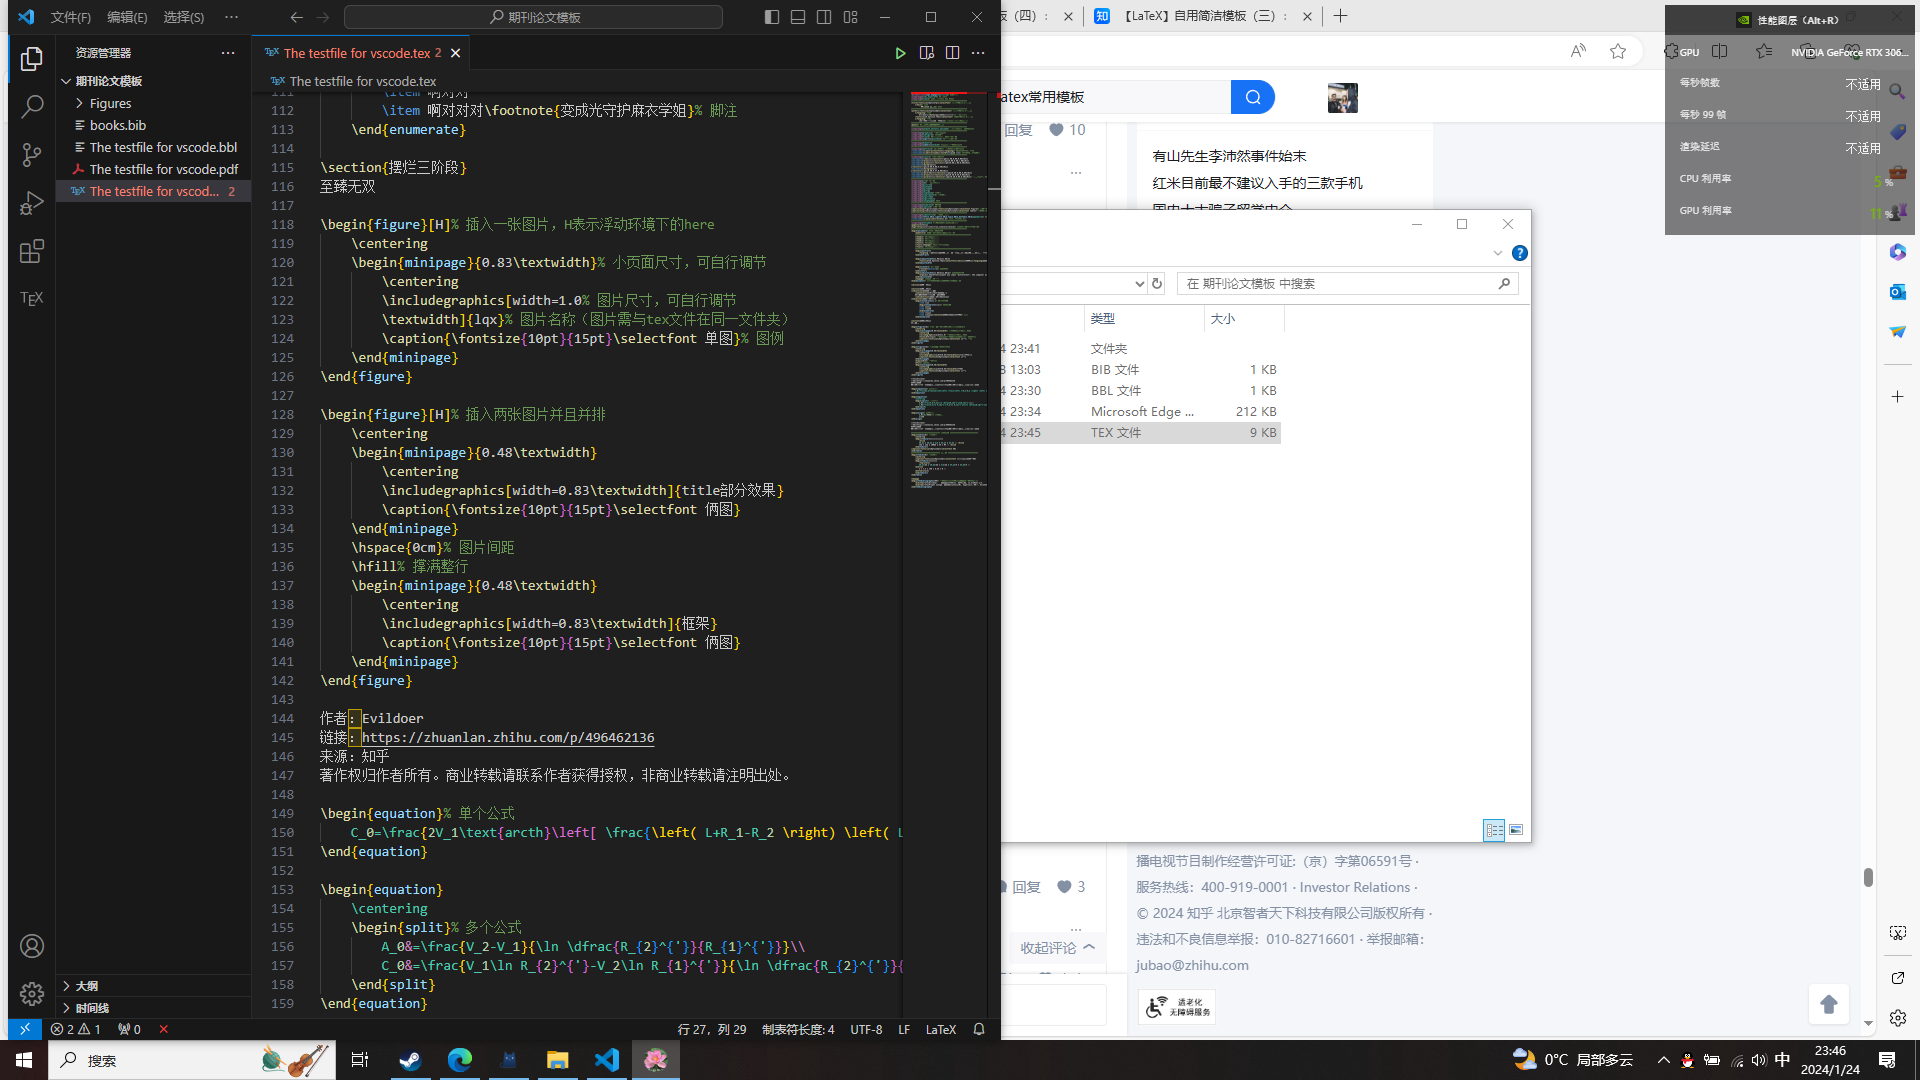
\includegraphics[width=1.0% 图片尺寸,可自行调节
		\textwidth]{1}% 图片名称(图片需与tex文件在同一文件夹)
		\caption{\fontsize{10pt}{15pt}\selectfont 单图}% 图例
	\end{minipage}
\end{figure}

\begin{figure}[H]% 插入两张图片并且并排
	\centering
	\begin{minipage}{0.48\textwidth}
		\centering
		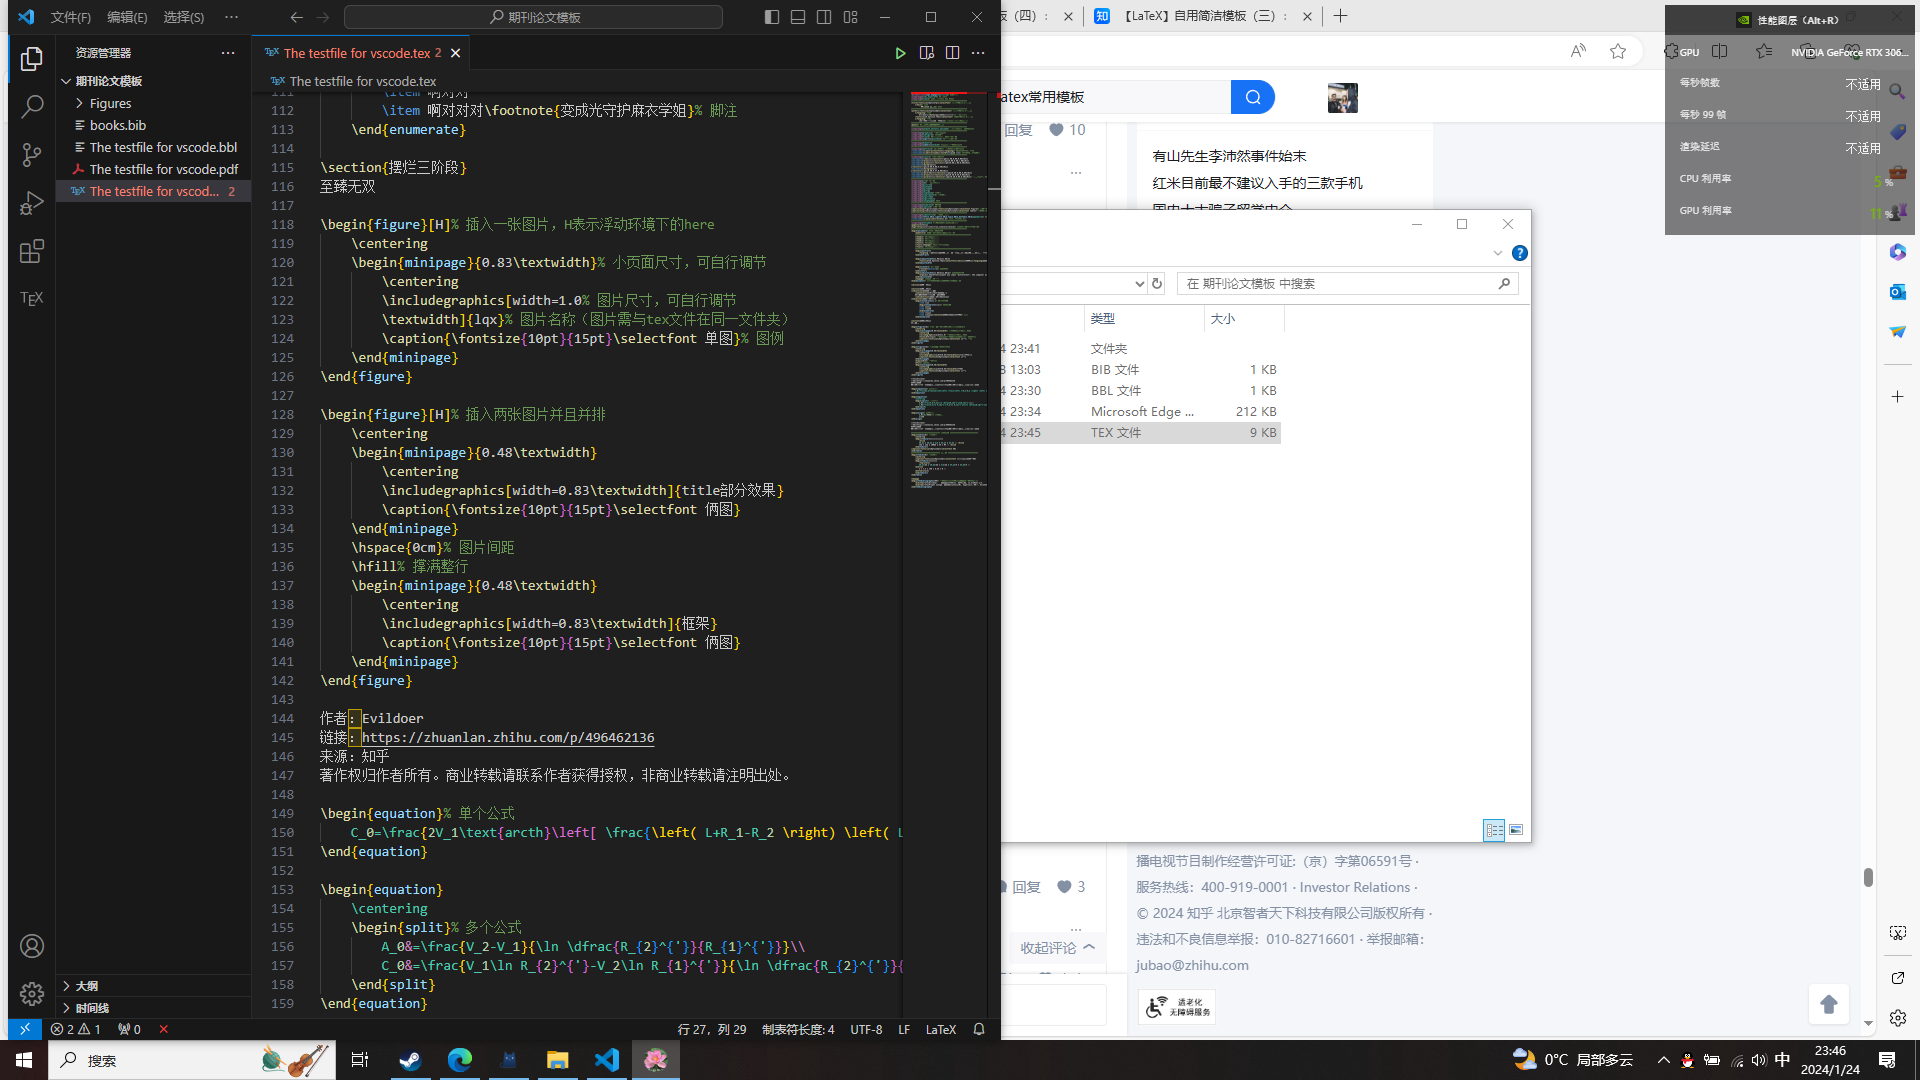
\includegraphics[width=0.83\textwidth]{1}
		\caption{\fontsize{10pt}{15pt}\selectfont 俩图}
	\end{minipage}
	\hspace{0cm}% 图片间距
	\hfill% 撑满整行
	\begin{minipage}{0.48\textwidth}
		\centering
		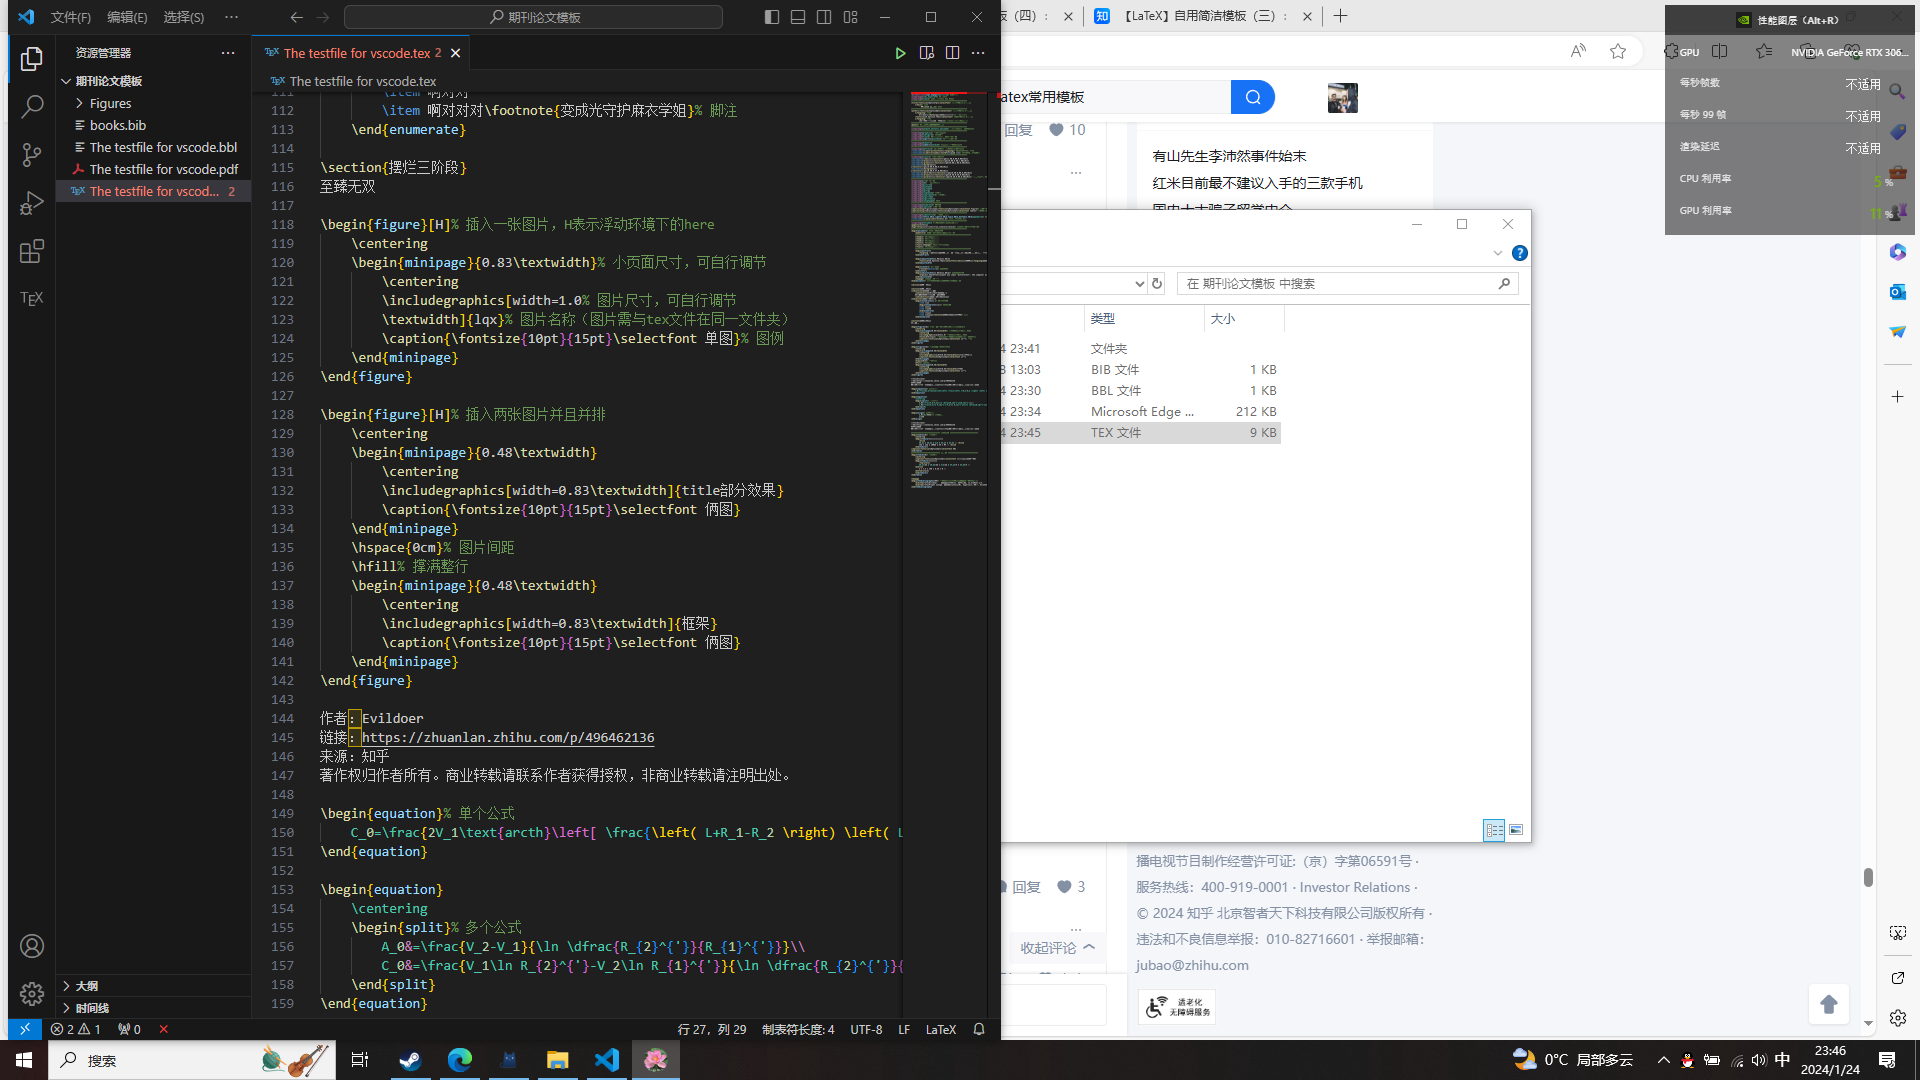
\includegraphics[width=0.83\textwidth]{1}
		\caption{\fontsize{10pt}{15pt}\selectfont 俩图}
	\end{minipage}
\end{figure}


\begin{equation}% 单个公式
	C_0=\frac{2V_1\text{arcth}\left[ \frac{\left( L+R_1-R_2 \right) \left( L-R_1-R_2 \right)}{\left( L+R_1+R_2 \right) \left( L-R_1+R_2 \right)} \right] ^{\frac{1}{2}}}{\text{arch}\left( \frac{L^2-R_{1}^{2}-R_{2}^{2}}{2R_1R_2} \right)}+\frac{2V_2\text{arcth}\left[ \frac{\left( L+R_2-R_1 \right) \left( L-R_1-R_2 \right)}{\left( L+R_1+R_2 \right) \left( L-R_2+R_1 \right)} \right] ^{\frac{1}{2}}}{\text{arch}\left( \frac{L^2-R_{1}^{2}-R_{2}^{2}}{2R_1R_2} \right)}
\end{equation}

\begin{equation}
	\centering
	\begin{split}% 多个公式
		A_0&=\frac{V_2-V_1}{\ln \dfrac{R_{2}^{'}}{R_{1}^{'}}}\\
		C_0&=\frac{V_1\ln R_{2}^{'}-V_2\ln R_{1}^{'}}{\ln \dfrac{R_{2}^{'}}{R_{1}^{'}}}
	\end{split}
\end{equation}

\begin{align}% 对齐公式
		A_0&=3c+6666\\% 注意换行
		&=369
\end{align}


%%%%%%%%%%%%%%%%%%%%%%%%%%%%% 网站给表 %%%%%%%%%%%%%%%%%%%%%%%%%%%%
\begin{table}[H]% 插入表格
	\centering
	\begin{tabular}{|l|l|l|l|l|}
		\hline
		$R_1$ & $R_2$ & $L$ & $V_1$ & $V_2$ \\ \hline
		1mm & 1mm & 100mm & 2V & 0V \\ \hline
	\end{tabular}
\caption{\fontsize{10pt}{15pt}\selectfont 表}
\end{table}

\newpage
\begin{thebibliography}{99}% 参考文献,{}内表示序号最大位数(两位)
	\bibitem{ref1}Evildoer. 开摆的深刻内涵[J]. 大学物理, 11.4(2022):1-4.
	\bibitem{ref2}Propht Joseph. 摆王的自我修养[M]. Supercell出版社, 01(2333):-2-$-\infty$.
\end{thebibliography}

\end{document}